\documentclass{standalone}
\usepackage{tikz}
\usetikzlibrary{patterns, positioning}
\usepackage[sfdefault]{ClearSans} %% option 'sfdefault' activates Clear Sans as the default text font
\usepackage[T1]{fontenc}

\begin{document}
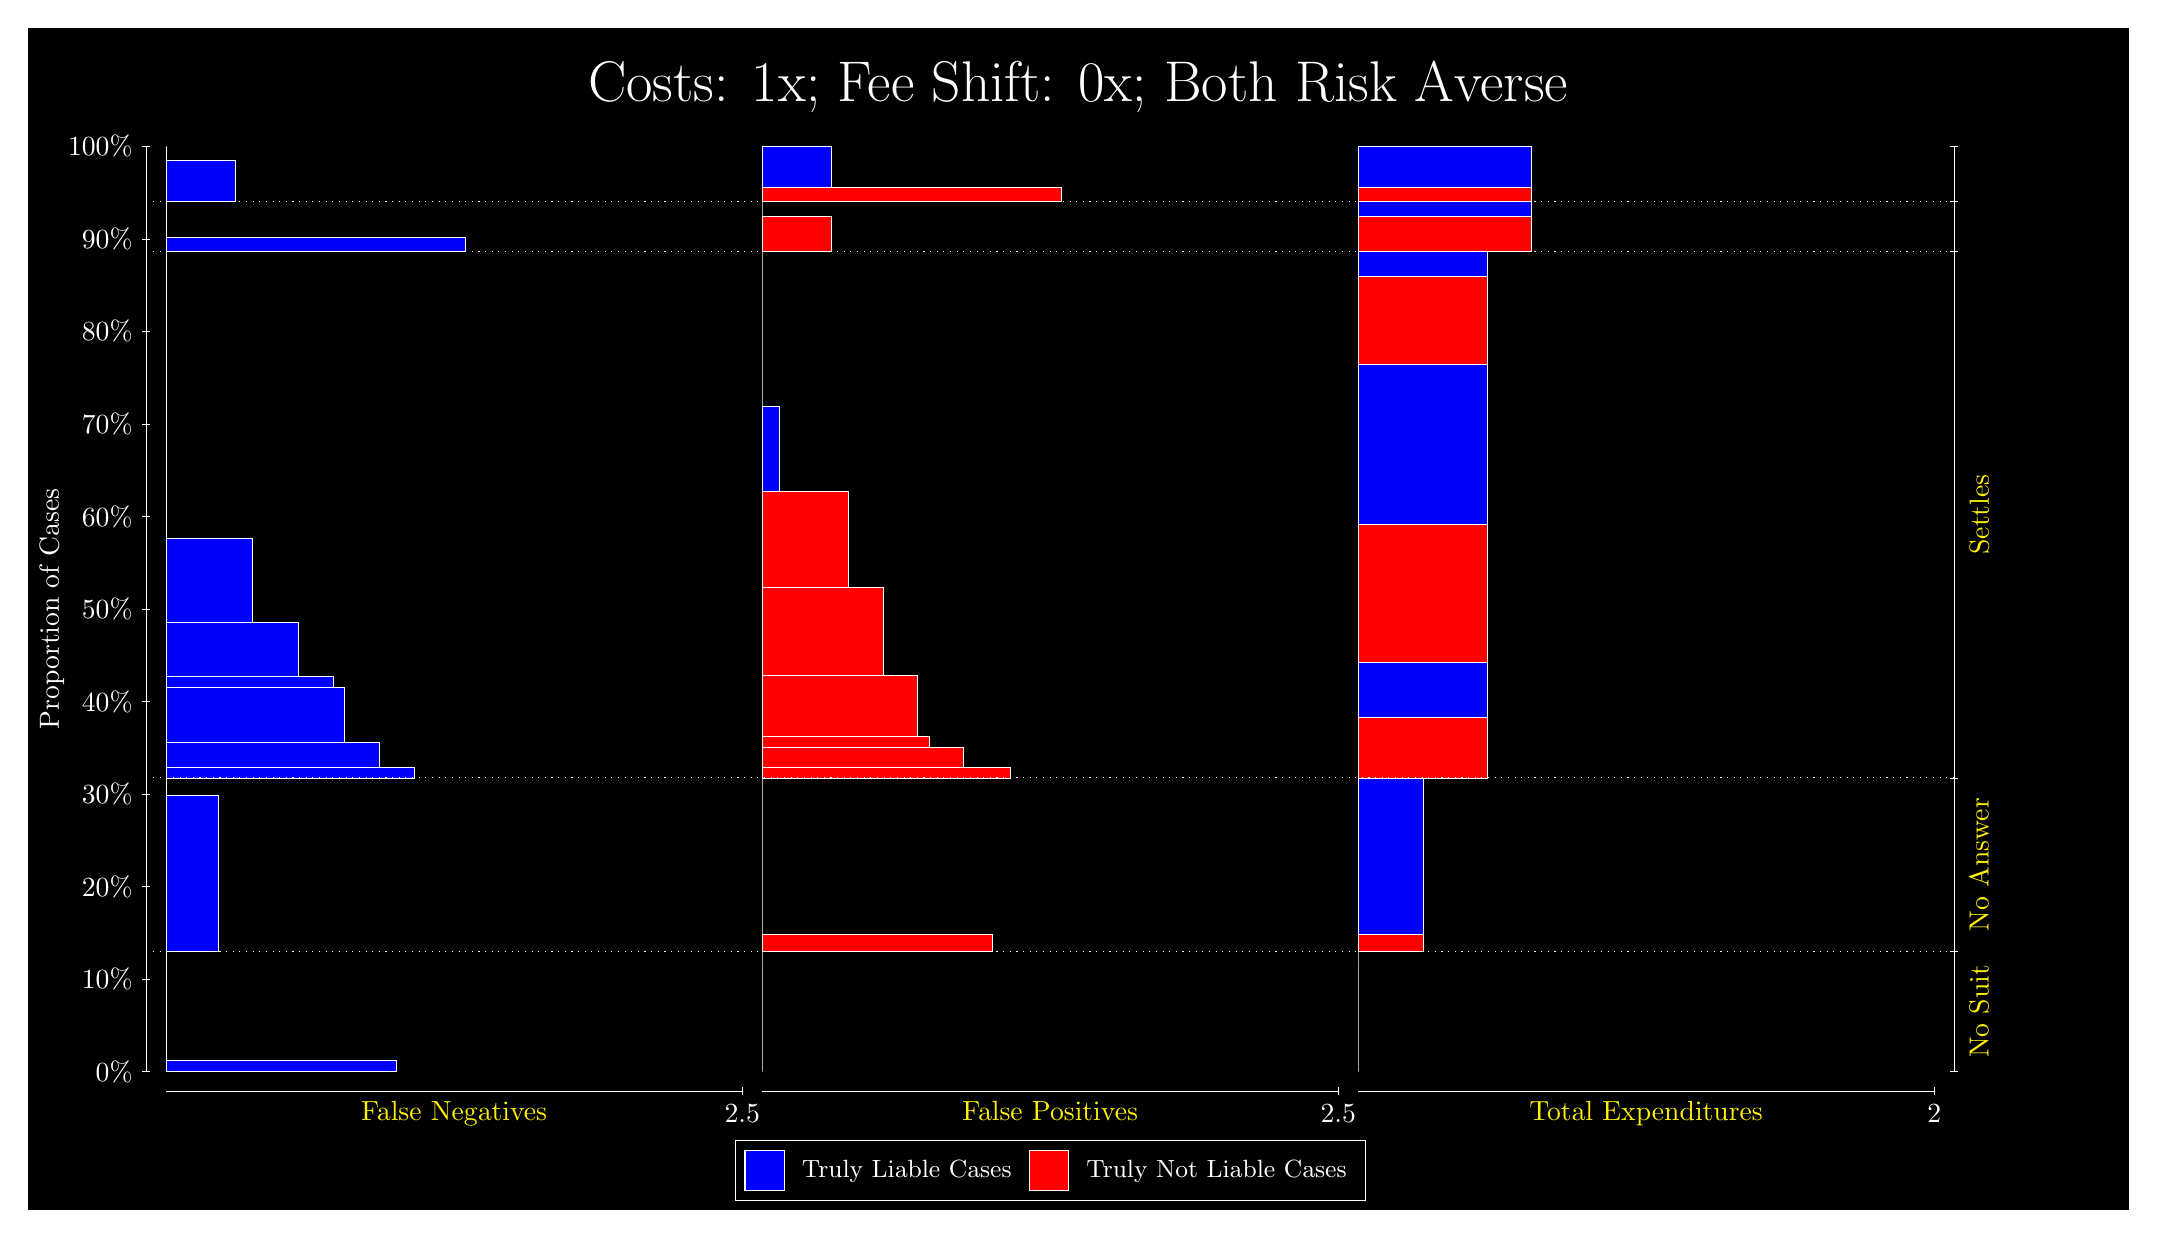
\begin{tikzpicture}
\draw[fill=black] (0,0) rectangle (26.667,15);
\draw[text=white] (0,13.5) rectangle (26.667,15) node[midway] {\huge Costs: 1x; Fee Shift: 0x; Both Risk Averse};
\draw[white, very thin] (1.5,1.75) -- (1.5,13.5);
\node[rotate=90, text=white, anchor=center] at (0.3, 7.625) {Proportion of Cases};
\draw[white, very thin] (1.45,1.75) -- (1.55,1.75);
\node[text=white, anchor=east] at (1.45, 1.75) {0\%};
\draw[white, very thin] (1.45,2.925) -- (1.55,2.925);
\node[text=white, anchor=east] at (1.45, 2.925) {10\%};
\draw[white, very thin] (1.45,4.1) -- (1.55,4.1);
\node[text=white, anchor=east] at (1.45, 4.1) {20\%};
\draw[white, very thin] (1.45,5.275) -- (1.55,5.275);
\node[text=white, anchor=east] at (1.45, 5.275) {30\%};
\draw[white, very thin] (1.45,6.45) -- (1.55,6.45);
\node[text=white, anchor=east] at (1.45, 6.45) {40\%};
\draw[white, very thin] (1.45,7.625) -- (1.55,7.625);
\node[text=white, anchor=east] at (1.45, 7.625) {50\%};
\draw[white, very thin] (1.45,8.8) -- (1.55,8.8);
\node[text=white, anchor=east] at (1.45, 8.8) {60\%};
\draw[white, very thin] (1.45,9.975) -- (1.55,9.975);
\node[text=white, anchor=east] at (1.45, 9.975) {70\%};
\draw[white, very thin] (1.45,11.15) -- (1.55,11.15);
\node[text=white, anchor=east] at (1.45, 11.15) {80\%};
\draw[white, very thin] (1.45,12.325) -- (1.55,12.325);
\node[text=white, anchor=east] at (1.45, 12.325) {90\%};
\draw[white, very thin] (1.45,13.5) -- (1.55,13.5);
\node[text=white, anchor=east] at (1.45, 13.5) {100\%};

\draw[white, very thin] (24.457,1.75) -- (24.457,13.5);
\draw[white, very thin] (24.407,1.75) -- (24.507,1.75);
\node[anchor=west] at (24.407, 1.75) {};
\draw[white, very thin] (24.407,3.2775) -- (24.507,3.2775);
\node[anchor=west] at (24.407, 3.2775) {};
\draw[white, very thin] (24.407,5.4805) -- (24.507,5.4805);
\node[anchor=west] at (24.407, 5.4805) {};
\draw[white, very thin] (24.407,12.165) -- (24.507,12.165);
\node[anchor=west] at (24.407, 12.165) {};
\draw[white, very thin] (24.407,12.799) -- (24.507,12.799);
\node[anchor=west] at (24.407, 12.799) {};
\draw[white, very thin] (24.407,13.5) -- (24.507,13.5);
\node[anchor=west] at (24.407, 13.5) {};

\draw[white, very thin, fill=blue] (1.75,1.75) rectangle (4.6775,1.8921);
\draw[white, very thin, fill=red] (1.75,1.8921) rectangle (1.75,3.2775);
\draw[white, very thin, fill=blue] (1.75,3.2775) rectangle (2.4087,5.2632);
\draw[white, very thin, fill=red] (1.75,5.2632) rectangle (1.75,5.4805);
\draw[white, very thin, fill=blue] (1.75,5.4805) rectangle (4.8971,5.6094);
\draw[white, very thin, fill=blue] (1.75,5.6094) rectangle (4.458,5.9279);
\draw[white, very thin, fill=blue] (1.75,5.9279) rectangle (4.0188,6.6295);
\draw[white, very thin, fill=blue] (1.75,6.6295) rectangle (3.8725,6.766);
\draw[white, very thin, fill=blue] (1.75,6.766) rectangle (3.4333,7.4501);
\draw[white, very thin, fill=blue] (1.75,7.4501) rectangle (2.8478,8.5265);
\draw[white, very thin, fill=red] (1.75,8.5265) rectangle (1.75,12.165);
\draw[white, very thin, fill=blue] (1.75,12.165) rectangle (5.5558,12.349);
\draw[white, very thin, fill=red] (1.75,12.349) rectangle (1.75,12.799);
\draw[white, very thin, fill=blue] (1.75,12.799) rectangle (2.6283,13.317);
\draw[white, very thin, fill=red] (1.75,13.317) rectangle (1.75,13.5);
\draw[white, very thin, fill=red] (9.3189,1.75) rectangle (9.3189,3.1354);
\draw[white, very thin, fill=blue] (9.3189,3.1354) rectangle (9.3189,3.2775);
\draw[white, very thin, fill=red] (9.3189,3.2775) rectangle (12.246,3.4948);
\draw[white, very thin, fill=blue] (9.3189,3.4948) rectangle (9.3189,5.4805);
\draw[white, very thin, fill=red] (9.3189,5.4805) rectangle (12.466,5.6168);
\draw[white, very thin, fill=red] (9.3189,5.6168) rectangle (11.88,5.862);
\draw[white, very thin, fill=red] (9.3189,5.862) rectangle (11.441,6.0088);
\draw[white, very thin, fill=red] (9.3189,6.0088) rectangle (11.295,6.7777);
\draw[white, very thin, fill=red] (9.3189,6.7777) rectangle (10.856,7.898);
\draw[white, very thin, fill=red] (9.3189,7.898) rectangle (10.417,9.1191);
\draw[white, very thin, fill=blue] (9.3189,9.1191) rectangle (9.5384,10.195);
\draw[white, very thin, fill=blue] (9.3189,10.195) rectangle (9.3189,12.165);
\draw[white, very thin, fill=red] (9.3189,12.165) rectangle (10.197,12.616);
\draw[white, very thin, fill=blue] (9.3189,12.616) rectangle (9.3189,12.799);
\draw[white, very thin, fill=red] (9.3189,12.799) rectangle (13.125,12.982);
\draw[white, very thin, fill=blue] (9.3189,12.982) rectangle (10.197,13.5);
\draw[white, very thin, fill=red] (16.888,1.75) rectangle (16.888,3.1354);
\draw[white, very thin, fill=blue] (16.888,3.1354) rectangle (16.888,3.2775);
\draw[white, very thin, fill=red] (16.888,3.2775) rectangle (17.711,3.4948);
\draw[white, very thin, fill=blue] (16.888,3.4948) rectangle (17.711,5.4805);
\draw[white, very thin, fill=red] (16.888,5.4805) rectangle (18.534,6.2494);
\draw[white, very thin, fill=blue] (16.888,6.2494) rectangle (18.534,6.9511);
\draw[white, very thin, fill=red] (16.888,6.9511) rectangle (18.534,8.7005);
\draw[white, very thin, fill=blue] (16.888,8.7005) rectangle (18.534,10.726);
\draw[white, very thin, fill=red] (16.888,10.726) rectangle (18.534,11.847);
\draw[white, very thin, fill=blue] (16.888,11.847) rectangle (18.534,12.165);
\draw[white, very thin, fill=red] (16.888,12.165) rectangle (19.083,12.616);
\draw[white, very thin, fill=blue] (16.888,12.616) rectangle (19.083,12.799);
\draw[white, very thin, fill=red] (16.888,12.799) rectangle (19.083,12.982);
\draw[white, very thin, fill=blue] (16.888,12.982) rectangle (19.083,13.5);
\draw[white, dotted] (1.5,3.2775) -- (24.457,3.2775);
\draw[white, dotted] (1.5,5.4805) -- (24.457,5.4805);
\draw[white, dotted] (1.5,12.165) -- (24.457,12.165);
\draw[white, dotted] (1.5,12.799) -- (24.457,12.799);
\draw[white, very thin] (1.75,1.5) -- (9.0689,1.5);
\node[text=yellow, anchor=north] at (5.4094, 1.5) {False Negatives};
\draw[white, very thin] (9.0689,1.45) -- (9.0689,1.55);
\node[text=white, anchor=north] at (9.0689, 1.45) {2.5};

\draw[white, very thin] (9.3189,1.5) -- (16.638,1.5);
\node[text=yellow, anchor=north] at (12.978, 1.5) {False Positives};
\draw[white, very thin] (16.638,1.45) -- (16.638,1.55);
\node[text=white, anchor=north] at (16.638, 1.45) {2.5};

\draw[white, very thin] (16.888,1.5) -- (24.207,1.5);
\node[text=yellow, anchor=north] at (20.547, 1.5) {Total Expenditures};
\draw[white, very thin] (24.207,1.45) -- (24.207,1.55);
\node[text=white, anchor=north] at (24.207, 1.45) {2};

\node[text=yellow, centered, rotate=90] at (24.777, 2.5137) {No Suit};
\node[text=yellow, centered, rotate=90] at (24.777, 4.379) {No Answer};
\node[text=yellow, centered, rotate=90] at (24.777, 8.8228) {Settles};



\draw (12.978300999999998,1.5) node[draw=none] (baseCoordinate) {};
\begin{scope}[align=center]
        \matrix[scale=0.5, draw=white, below=0.5cm of baseCoordinate, nodes={draw}, column sep=0.1cm]{
            \node[rectangle, draw, minimum width=0.5cm, minimum height=0.5cm, fill=blue] {}; &
            \node[draw=none, font=\small, text=white] (B) {Truly Liable Cases}; &
            \node[rectangle, draw, minimum width=0.5cm, minimum height=0.5cm, fill=red] {}; &
            \node[draw=none, font=\small, text=white] (B) {Truly Not Liable Cases}; \\
            };
\end{scope}

\end{tikzpicture}
\end{document}